\section{Data Exploration \& Descriptive Analytics}

\subsection{Data Exploration}

The COVID-19 Dataset~\parencite[]{2023:NizMei}, provides a comprehensive view of the impact
of the COVID-19 pandemic focusing on various aspects of the patients such as:
\begin{itemize}
    \item Hospitalization;
    \item Symptoms;
    \item Medical Records.
\end{itemize}
This dataset is useful to \emph{identify high risk factors and predict hospitalizations}.
It also contains extensive anonymized data related to patients with their conditions. It features
\emph{21 different attributes} and \emph{1,048,575 unique patient records}.

Boolean features are identified by $1$ meaning `yes' and $2$ meaning `no'. Missing data is specified
out-of-range values like $97$ to $99$ or $9999$.

\subsection{Features Description}

So the features provided from the dataset provides a comprehensive profile of 
patient health status and the medical care received. You can find a deep analysis per feature
in the appendix section~\nameref{app:features-analysis-in-depth}.

In terms of null values, we have a minimal number of empty entries (always close to 0\%), except 
when the data does not make sense. For example, in the case of pregnancy, we have 50\% missing 
data. This is reasonable because half of the dataset consists of men. In the case of intubation 
or ICU data, there is 82\% missing data. This is likely because the majority of the patients
were not hospitalized.

You can get all the statistics resume in the Figure~\ref{fig:feature_summary}.

\subsection{Insights}

\subsubsection{Age}

Age appears to be one of the primary factors in determining whether a patient will be hospitalized 
or survive COVID-19.

As you age, you become more susceptible to various diseases, and your immune system weakens, 
increasing the likelihood of experiencing severe complications if you contract COVID-19. 
(Figure~\ref{fig:age_insights_resume} and Figure~\ref{fig:age_insights}).

\begin{figure}[H]%
    \caption{Age by Disease}%
    \label{fig:age_insights_resume}%
    \centering
    \subfloat[\centering Hypertension]{{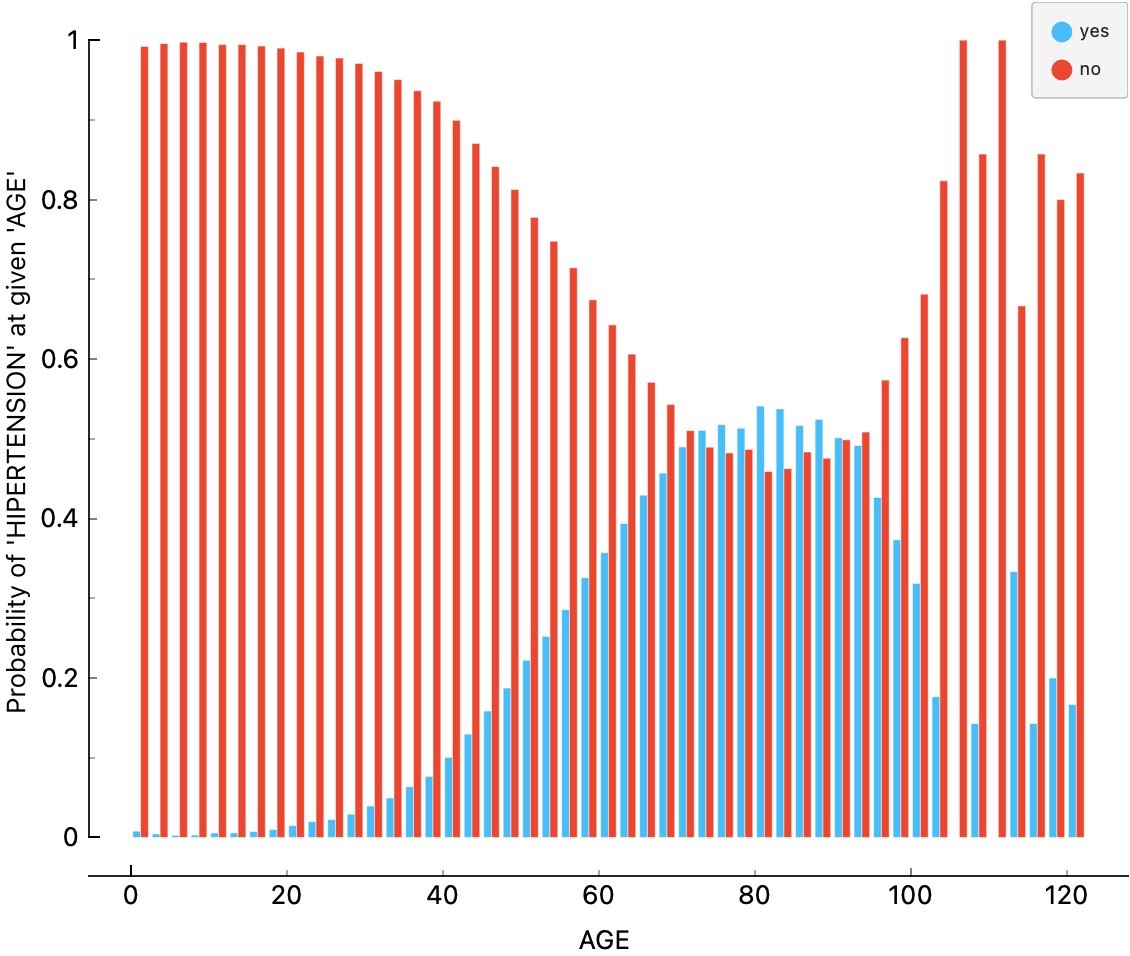
\includegraphics[width=0.40\textwidth]{img/appendix/insight_age_hipertension.png} }}%
    \qquad
    \subfloat[\centering Pneumonia]{{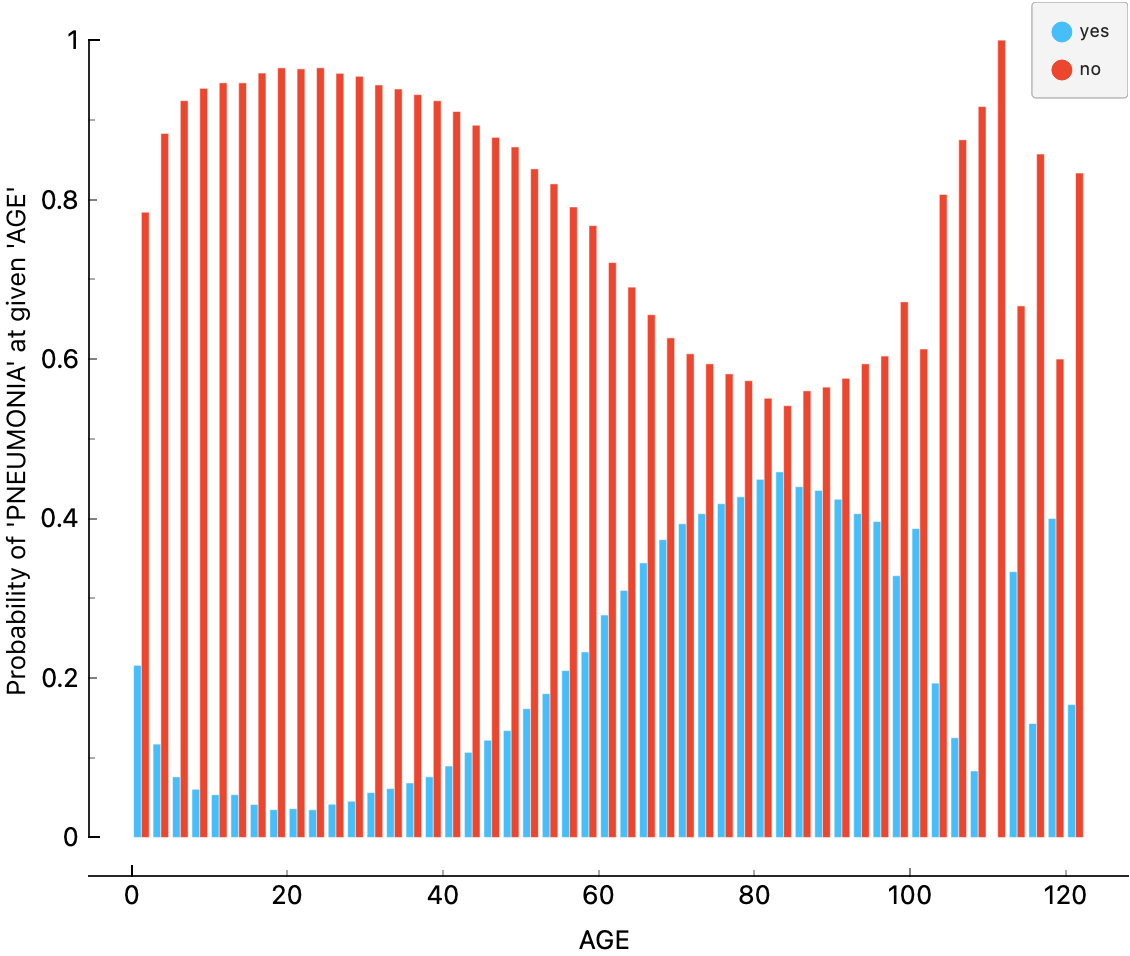
\includegraphics[width=0.40\textwidth]{img/appendix/insight_age_pneumonia.png} }}%
\end{figure}

Additionally, older individuals are more likely to experience the following 
outcomes if they contract COVID-19:
\begin{itemize}
    \item Being Hospitalized;
    \item Being Intubated;
    \item Dying.
\end{itemize}

\begin{figure}[H]%
    \caption{Age by Outcome}%
    \label{fig:age_insights_outcome}%
    \centering
    \subfloat[\centering Died]{{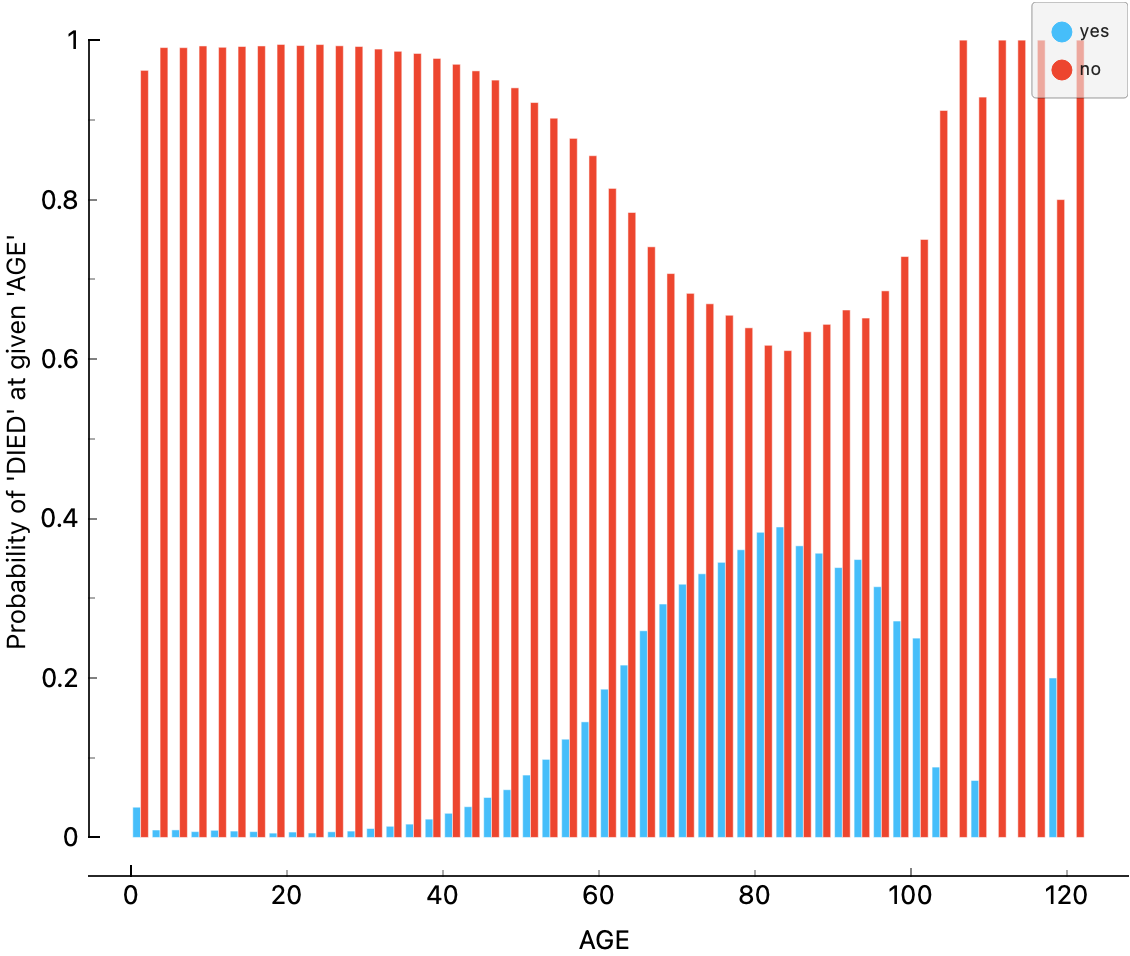
\includegraphics[width=0.40\textwidth]{img/dataexploration/insight_age_died.png} }}%
    \qquad
    \subfloat[\centering Intubated]{{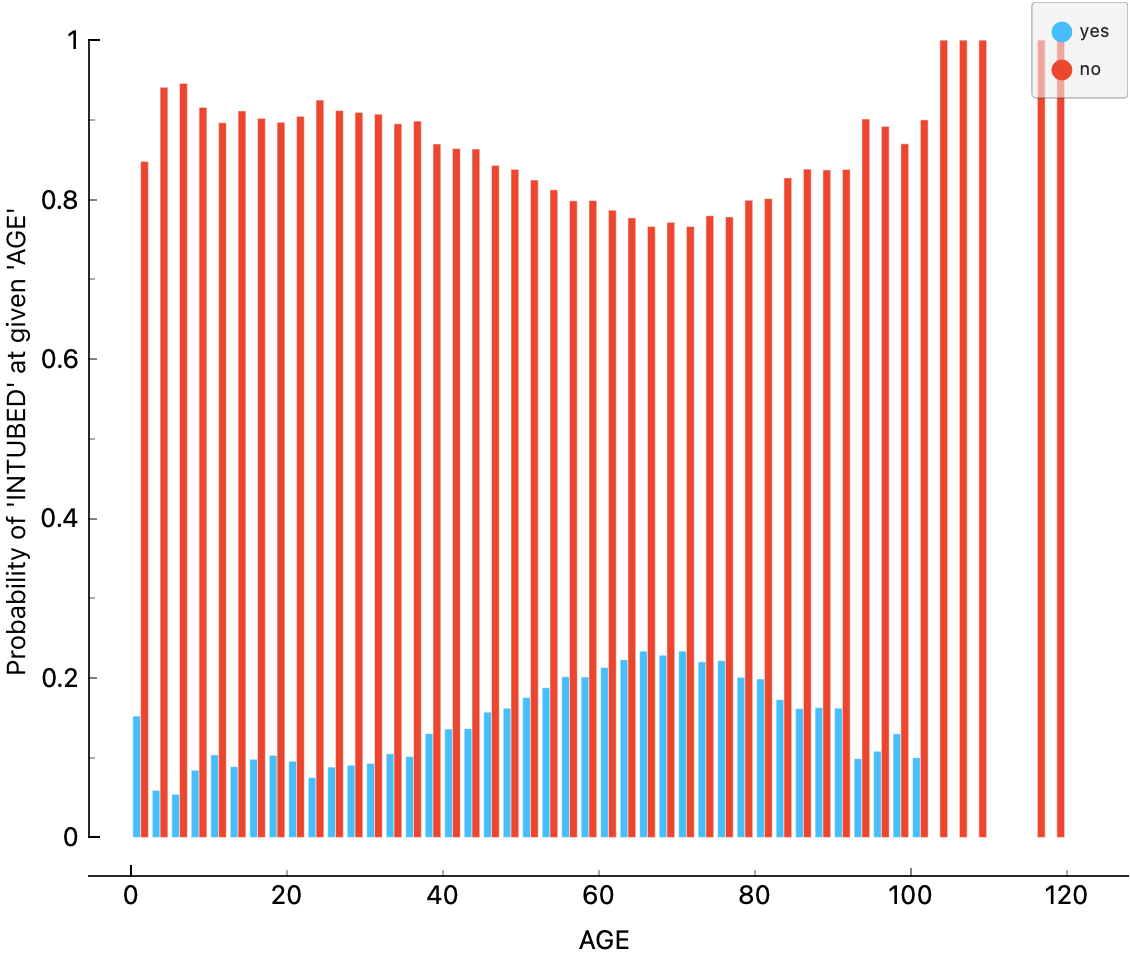
\includegraphics[width=0.40\textwidth]{img/dataexploration/insight_age_intubated.png} }}%
    \qquad
    \subfloat[\centering Hospitalized]{{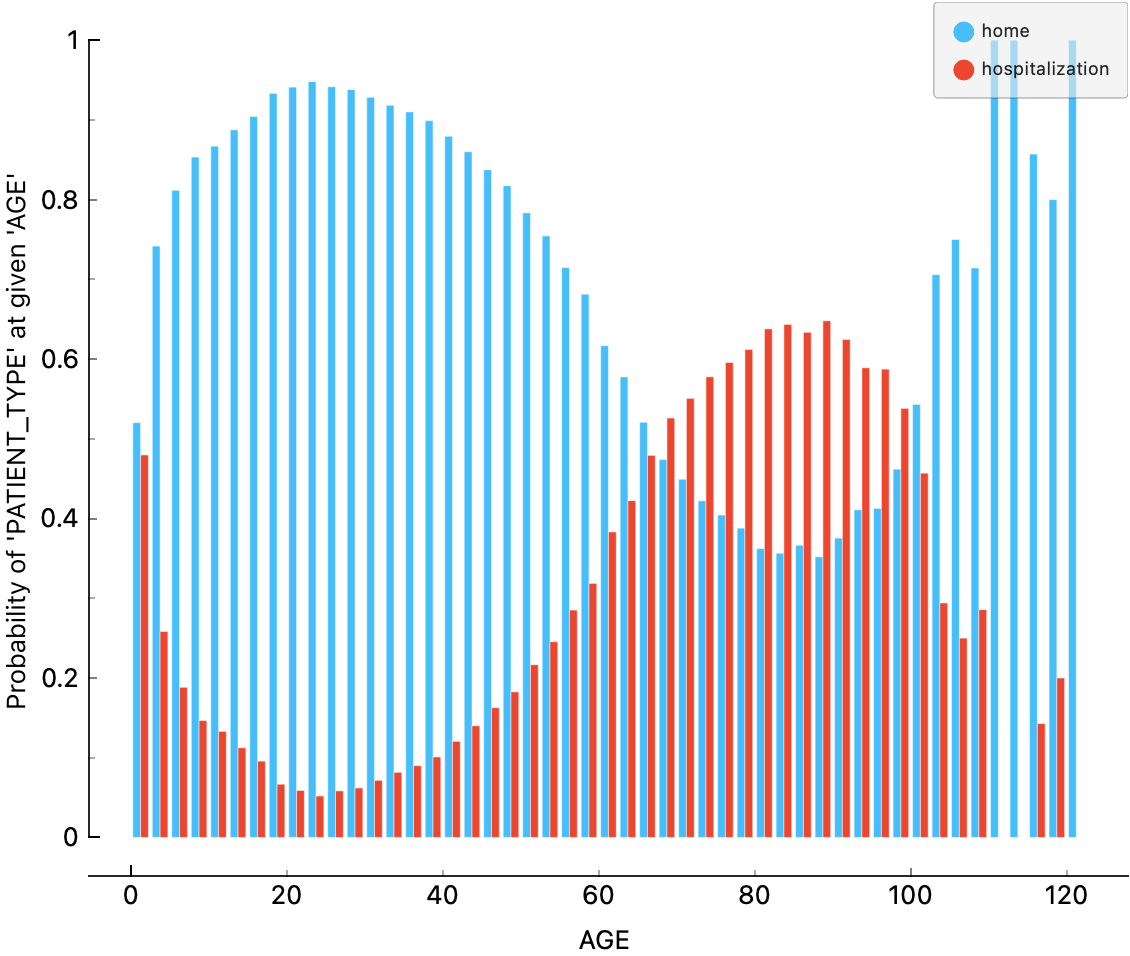
\includegraphics[width=0.40\textwidth]{img/dataexploration/insight_age_hospitalization.png} }}%
\end{figure}

\subsubsection{Pneumonia}

Pneumonia significantly complicates the condition of COVID-19 patients, often
leading to more severe symptoms and outcomes. Effective management and early 
intervention are crucial to mitigate the adverse effects associated with pneumonia
in these patients.

\begin{figure}[H]%
    \caption{Pneumonia by Outcome}%
    \label{fig:pneumonia_insights_outcome}%
    \centering
    \subfloat[\centering Died]{{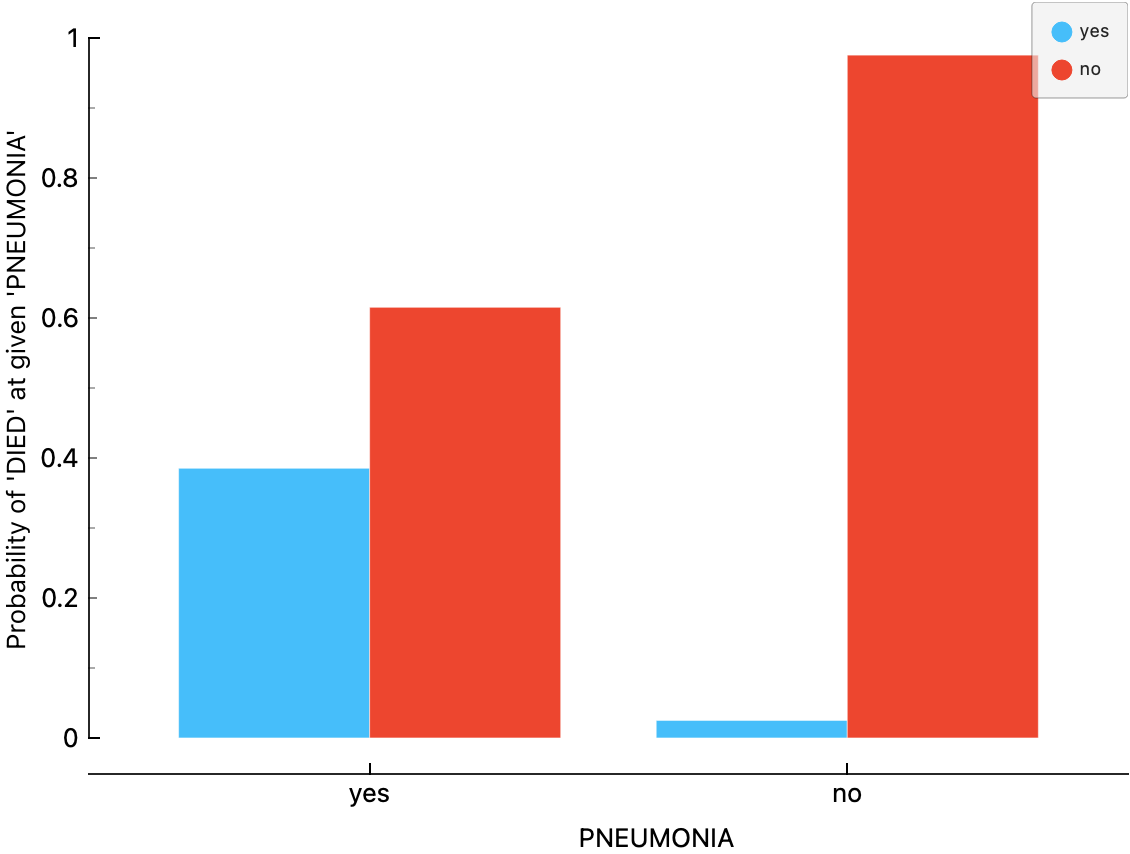
\includegraphics[width=0.29\textwidth]{img/dataexploration/insight_pneumonia_died.png} }}%
    \qquad
    \subfloat[\centering Intubated]{{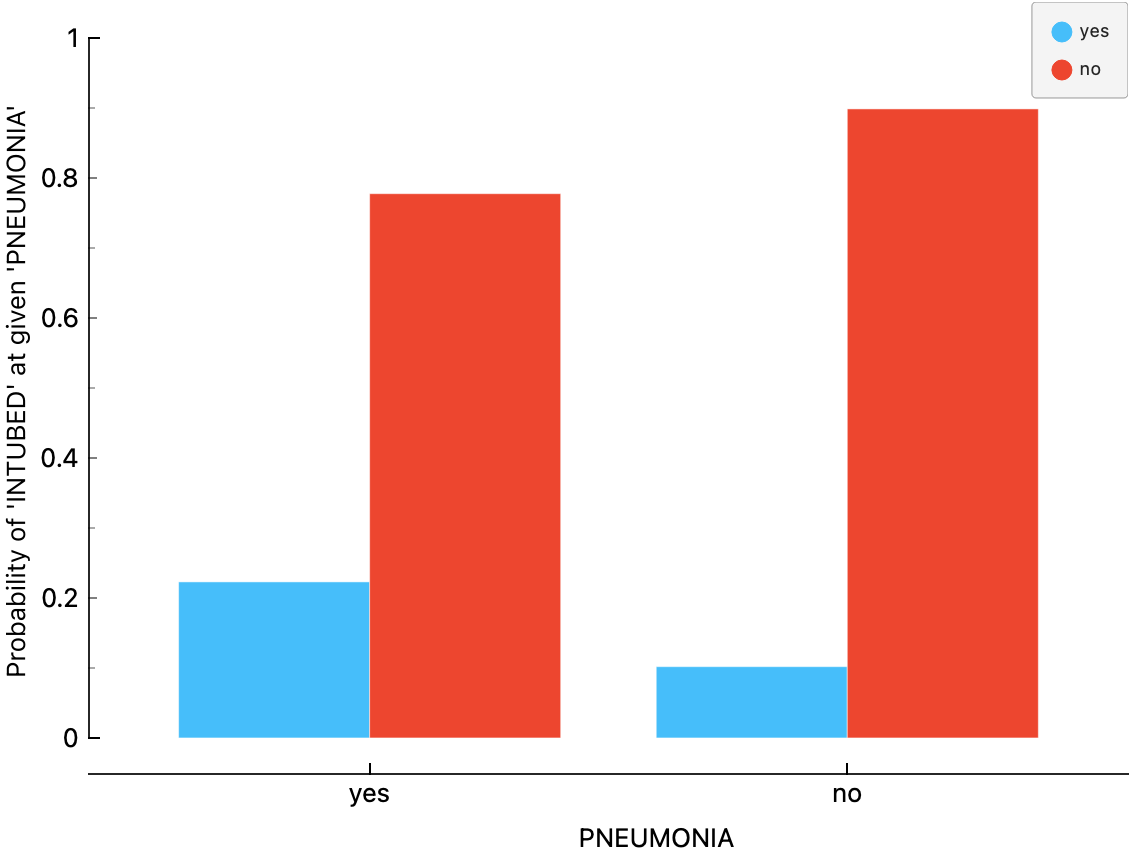
\includegraphics[width=0.29\textwidth]{img/dataexploration/insight_pneumonia_intubed.png} }}%
    \qquad
    \subfloat[\centering Hospitalized]{{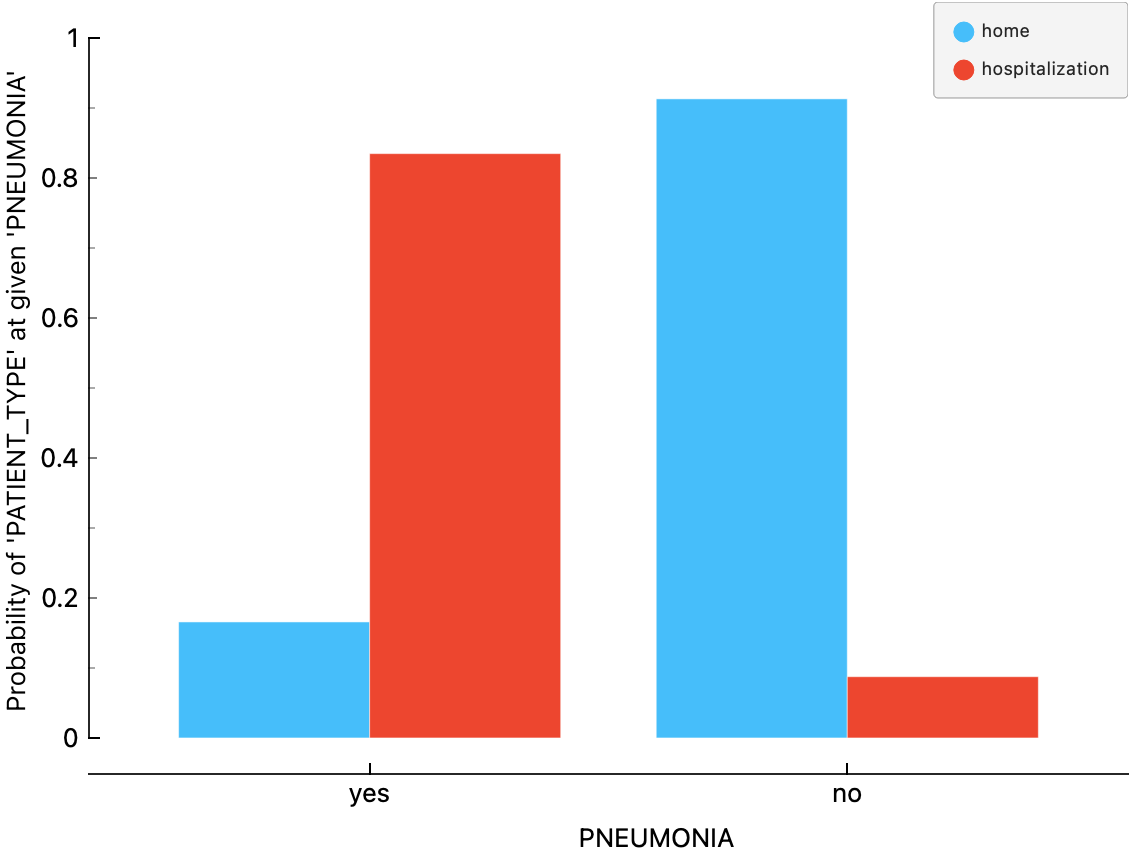
\includegraphics[width=0.29\textwidth]{img/dataexploration/insight_pneumonia_patient_type.png} }}%
\end{figure}

\subsection{Intubation and ICU}

Patients with COVID-19 who require intubation or admission to an intensive care unit
(ICU) are generally at a higher risk of mortality compared to those who do not
require such intensive interventions.

\begin{figure}[H]%
    \caption{Intubation and ICU vs Death}%
    \label{fig:intubation_insights_outcome}%
    \centering
    \subfloat[\centering Intubated]{{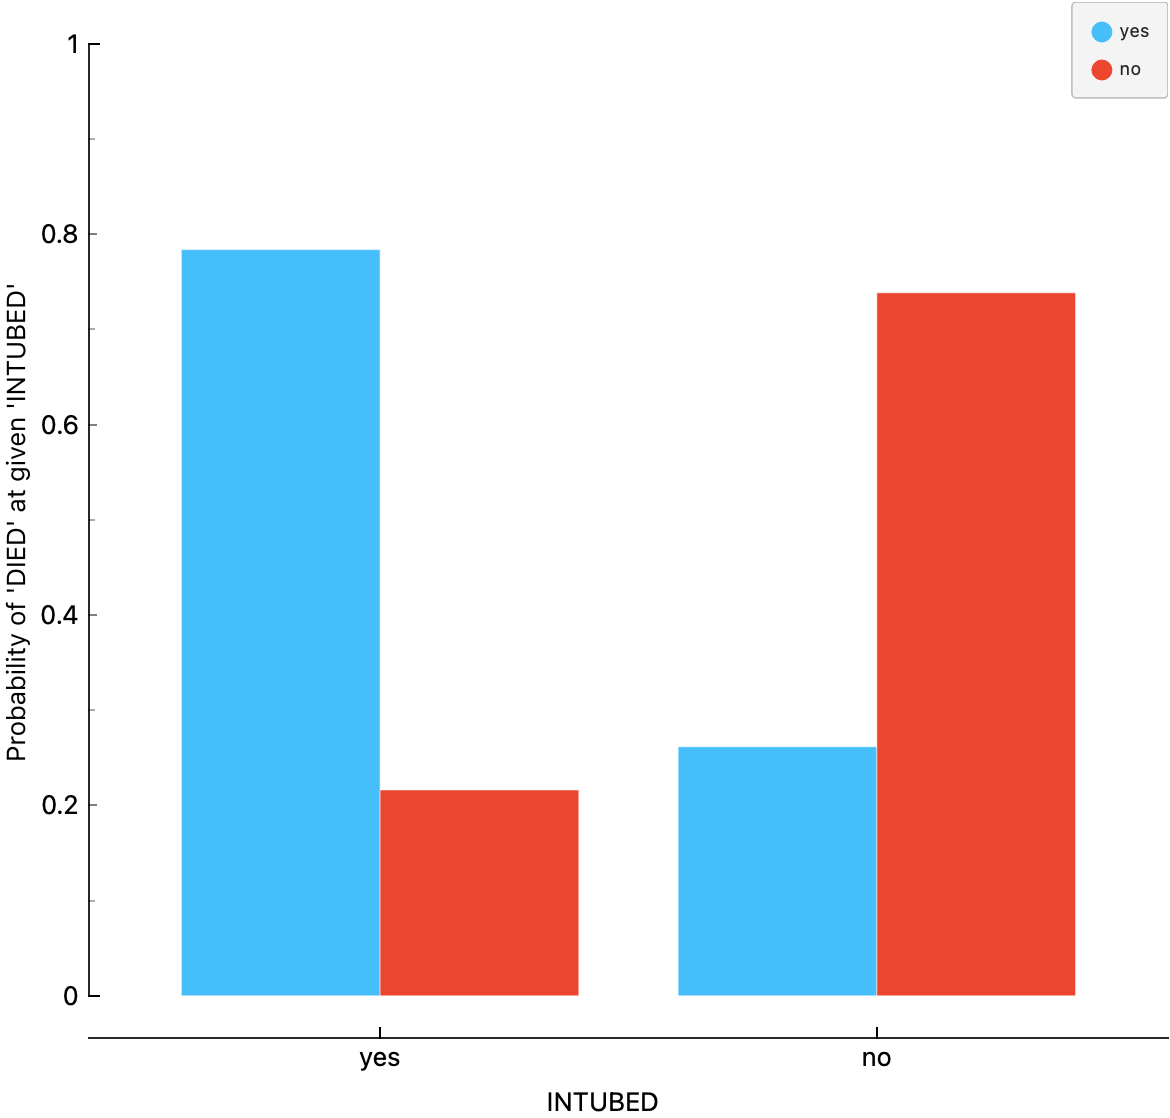
\includegraphics[width=0.40\textwidth]{img/dataexploration/insight_intubed_died.png} }}%
    \qquad
    \subfloat[\centering ICU]{{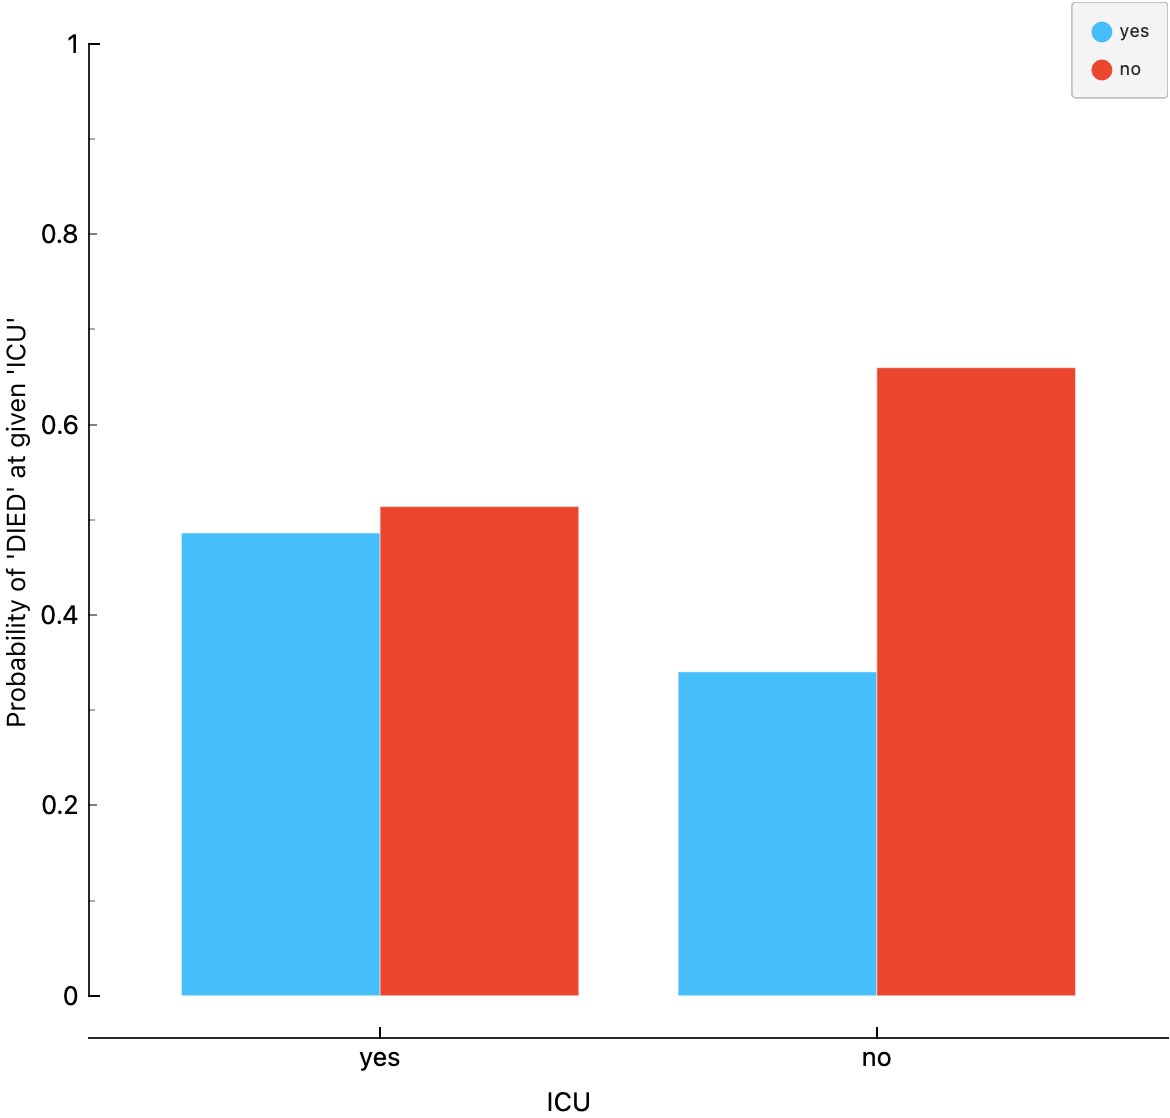
\includegraphics[width=0.40\textwidth]{img/dataexploration/insight_icu_died.png} }}%
\end{figure}

\subsection{Other observations}

You can discover insights by creating and examining the correlation matrix among features. An intriguing observation from the matrix suggests that if you have one condition, such as renal disease or diabetes, you are also likely to have other related conditions.

Observing the correlation matrix, these are the most significant (Figure~\ref{fig:feat_corr_matrix}):
\begin{itemize}
    \item Only women are pregnant;
    \item Only if you are hospitalized and in ICU you can be intubed;
    \item Only if you are hospitalized we can be in ICU;
    \item There are some correlation between the conditions: (Obesity, COPD and Diabetes) and others.
\end{itemize}





